\documentclass[unicode,11pt,a4paper,oneside,numbers=endperiod,openany]{scrartcl}
\usepackage{amsmath}
\usepackage{float}  % To prevent floating of figures
\usepackage{lmodern}
\usepackage{listings}
\usepackage{hyperref}
\usepackage[utf8]{inputenc}  % Allows UTF-8 input (for special characters, etc.)
\usepackage{amsmath}         % Provides advanced math features
\usepackage{amssymb}         % For additional math symbols
\usepackage{graphicx}        % Allows including images
\usepackage{array}           % For tables
\usepackage{geometry}        % To adjust page margins
\usepackage{hyperref}        % For links and references
\usepackage{fancyhdr}        % For customized headers and footers
\usepackage{multicol}        % For multiple columns
\usepackage{verbatim}        % For verbatim text (like the gene sequence)
\usepackage{longtable}       % For long tables that span multiple pages
\usepackage{xcolor}          % For colored text (if needed)
\usepackage{listings}
\usepackage{dnaseq}         % For DNA sequences
\usepackage{amsmath}
\usepackage{float}  % To prevent floating of figures
\usepackage{lmodern}
\usepackage{listings}
\usepackage{pdfpages}
\usepackage{booktabs}  % Add this line to include the booktabs package
\usepackage{ifthen}
\usepackage[utf8]{inputenc}
\usepackage{graphics}
\usepackage{graphicx}
\usepackage{hyperref}

\pagestyle{plain}
\voffset -5mm
\oddsidemargin  0mm
\evensidemargin -11mm
\marginparwidth 2cm
\marginparsep 0pt
\topmargin 0mm
\headheight 0pt
\headsep 0pt
\topskip 0pt        
\textheight 255mm
\textwidth 165mm

\newcommand{\duedate} {}
\newcommand{\setduedate}[1]{%
\renewcommand\duedate {See iCorsi for due date}}
\newcommand\isassignment {false}
\newcommand{\setassignment}{\renewcommand\isassignment {true}}
\newcommand{\ifassignment}[1]{\ifthenelse{\boolean{\isassignment}}{#1}{}}
\newcommand{\ifnotassignment}[1]{\ifthenelse{\boolean{\isassignment}}{}{#1}}

\newcommand{\assignmentpolicy}{
\begin{table}[h]
\begin{center}
\scalebox{0.8} {%
\begin{tabular}{|p{0.02cm}p{16cm}|}
\hline
&\\
\multicolumn{2}{|c|}{\Large\textbf{HPC Lab ---  Submission Instructions}}\\
\multicolumn{2}{|c|}{\large\textbf{(Please, notice that following instructions are mandatory: }}\\
\multicolumn{2}{|c|}{\large\textbf{submissions that don't comply with, won't be considered)}}\\
&\\
\textbullet & Assignments must be submitted to \href{https://www.icorsi.ch}{iCorsi} (i.e. in electronic format).\\
\textbullet & Provide both executable package and sources (e.g. C/C++ files, Matlab). 
If you are using libraries, please add them in the file. Sources must be organized in directories called:\\
\multicolumn{2}{|c|}{\textit{Project\_number\_lastname\_firstname}}\\
& and  the  file must be called:\\
\multicolumn{2}{|c|}{\textit{project\_number\_lastname\_firstname.zip}}\\
\multicolumn{2}{|c|}{\textit{project\_number\_lastname\_firstname.pdf}}\\
\textbullet &  The TAs will grade your project by reviewing your project write-up, and looking at the implementation 
                 you attempted, and benchmarking your code's performance.\\

\textbullet & You are allowed to discuss all questions with anyone you like; however: (i) your submission must list anyone you discussed problems with and (ii) you must write up your submission independently.\\
\hline
\end{tabular}
}
\end{center}
\end{table}
}
\newcommand{\punkte}[1]{\hspace{1ex}\emph{\mdseries\hfill(#1~\ifcase#1{Points}\or{Points}\else{Points}\fi)}}


\newcommand\serieheader[6]{
\thispagestyle{empty}%
\begin{flushleft}

\includegraphics[width=0.4\textwidth]{usi_inf.png}
\end{flushleft}
  \noindent%
  {\large\ignorespaces{\textbf{#1}}\hspace{\fill}\ignorespaces{ \textbf{#2}}}\\ \\%
  {\large\ignorespaces #3 \hspace{\fill}\ignorespaces #4}\\
  \noindent%
  \bigskip
  \hrule\par\bigskip\noindent%
  \bigskip {\ignorespaces {\Large{\textbf{#5}}}
  \hspace{\fill}\ignorespaces \large \ifthenelse{\boolean{\isassignment}}{\duedate}{#6}}
  \hrule\par\bigskip\noindent%  \linebreak
 }

\makeatletter
\def\enumerateMod{\ifnum \@enumdepth >3 \@toodeep\else
      \advance\@enumdepth \@ne
      \edef\@enumctr{enum\romannumeral\the\@enumdepth}\list
      {\csname label\@enumctr\endcsname}{\usecounter
        {\@enumctr}%%%? the following differs from "enumerate"
	\topsep0pt%
	\partopsep0pt%
	\itemsep0pt%
	\def\makelabel##1{\hss\llap{##1}}}\fi}
\let\endenumerateMod =\endlist
\makeatother




\usepackage{textcomp}







\lstset{
  language=C++,                     % Set language to Python
  basicstyle=\ttfamily\footnotesize,   % Basic font style for the code
  keywordstyle=\bfseries\color{blue},  % Keywords in bold blue
  commentstyle=\color{gray},          % Comments in green
  stringstyle=\color{orange},          % Strings in orange
  showstringspaces=false,              % Don't show spaces in strings
  frame=single,                        % Adds a frame around the code
  numbers=left,                        % Line numbers on the left
  numberstyle=\tiny\color{gray},       % Line number style
  breaklines=true,                     % Allows breaking long lines
  tabsize=4                            % Sets default tab size
}


\begin{document}


\setassignment

\serieheader{High-Performance Computing Lab}{Institute of Computing}{Student: Jonatan Bella}{Discussed with: None}{Solution for Project 4}{}
\newline

\assignmentpolicy

\section{Task: Ring Sum using MPI [10 Points]}
For this implementation, first I defined the starting sum value of the process to be the rank number since
it would be the first element to be sum in each case. I provide a draft with the idea as I thought how to implement it:

\begin{figure}[H]
    \centering
    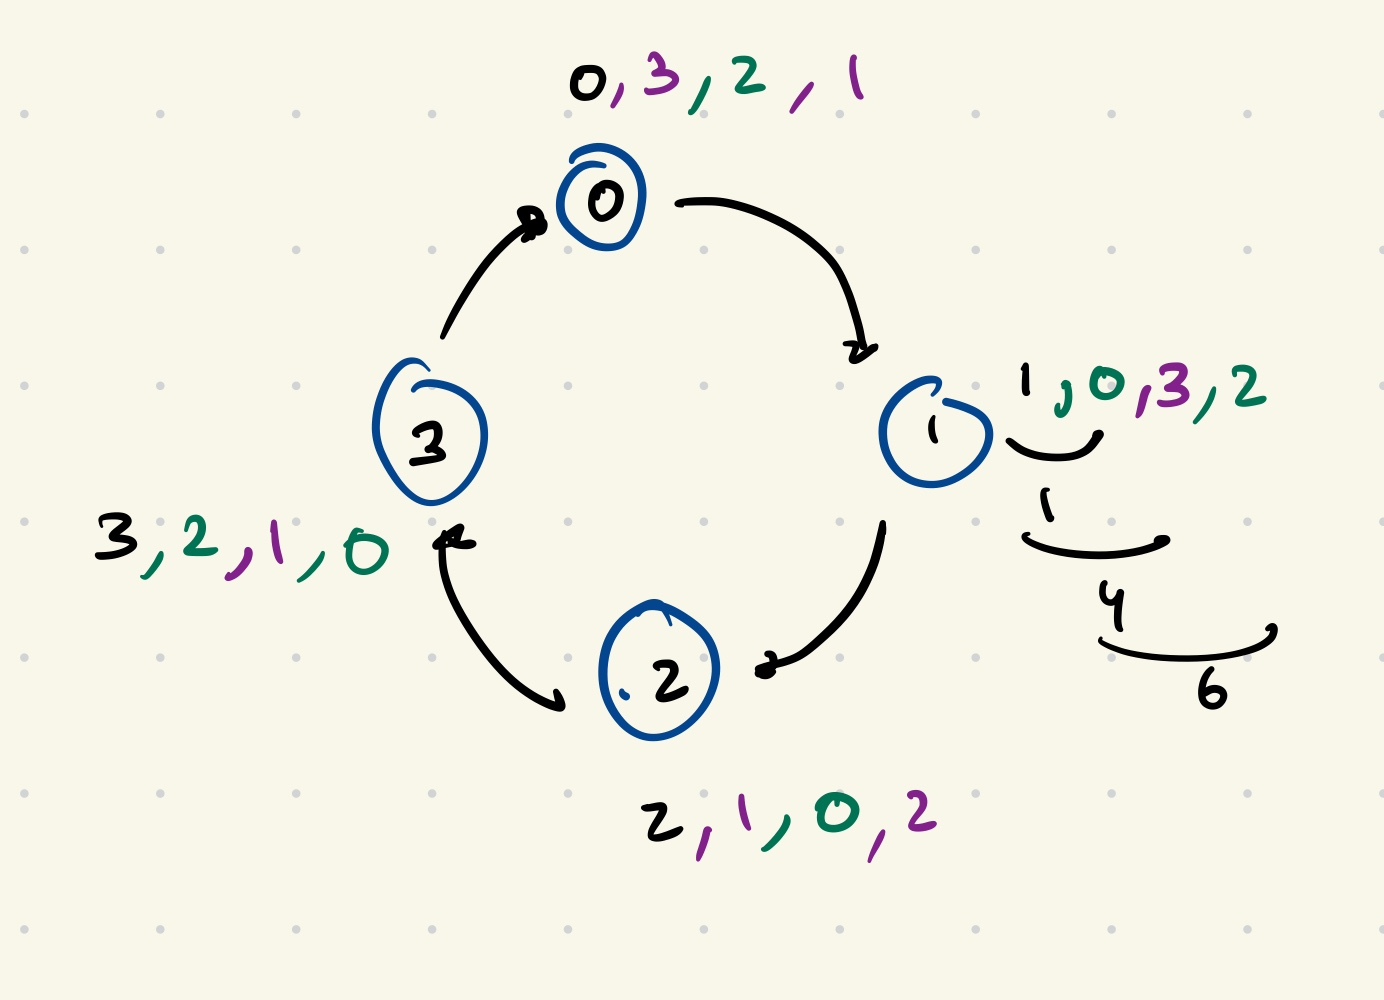
\includegraphics[width=\textwidth]{./img/exe1/idea.jpeg}
    \caption{Draft of the implementation}
  \end{figure}

Then, we need to calculate the next and previous ranks to each node since we need to pass the destination and source to the $MPI_Send$ and $MPI_Recv$ functions respectively. 
For this, we can use the modulo operation since the ranks are cyclic:

\begin{verbatim}
    int next = (rank + 1) % size;
    int prev = (rank - 1 + size) % size;
\end{verbatim}

The first case allows us to manage for the edge case of the last rank ($last\_rank + 1 = size$, therefore $next = 0$, which is the initial rank) and the second one for the first rank ($first\_rank - 1 = -1$, therefore $prev = size - 1$, which is the last rank).

Then, as mentioned in the assignment, we create a sender message variable to firstly send the rank of the node and then another one for receiving the sent message.

Now, we loop over the size of the nodes / processes taking into account, as indicated in assignment, the possibility of a deadlock. 
Therefore, we can add a condition such that if the rank is even, then first send the message then receives. Whereas, if odd, first receives then sends.
This for sure would avoid any deadlock since the neighbors of each node would be even for an odd case and vice versa.

After the first iteration is complete, the initial rank was sent and the next message would be the last received one
(this can be visualized with the green and violet colors in the draft). This is repeated until all the nodes have received the message, and we iterated
over all the processes ($size - 1$ times).
Interestingly, I thought we would have the same problem as in the provided example of $point-to-point$ in class, where the 
program would get stuck in a deadlock if the order of send and receiving is not managed. However, when I test this code without the conditions,
it actually worked anyway. I don't know if MPI manage this somehow, but I stick with the described implementation since it makes more sense to me. 

\begin{verbatim}
    for (int i = 0; i < size-1; i++) {
        if (rank % 2 == 0) { 
          MPI_Send(&send_message, 1, MPI_INT, next, 0, MPI_COMM_WORLD); 
          MPI_Recv(&recv_message, 1, MPI_INT, prev, 0, MPI_COMM_WORLD, MPI_STATUS_IGNORE);
        } else {
          MPI_Recv(&recv_message, 1, MPI_INT, prev, 0, MPI_COMM_WORLD, MPI_STATUS_IGNORE);
          MPI_Send(&send_message, 1, MPI_INT, next, 0, MPI_COMM_WORLD);
        }
        sum += recv_message; 
        send_message = recv_message;
      }
\end{verbatim}

\footnote{
    Sources: 
\url{https://hpc-tutorials.llnl.gov/mpi/routine_args/}
\newline 
$point-to-point$ class example
}

\section{Task: Ghost cells exchange between neighboring processes [15 Points]}

To implement the required solution, i first present the draft with a summary of my reasoning:

\begin{figure}[H]
    \centering
    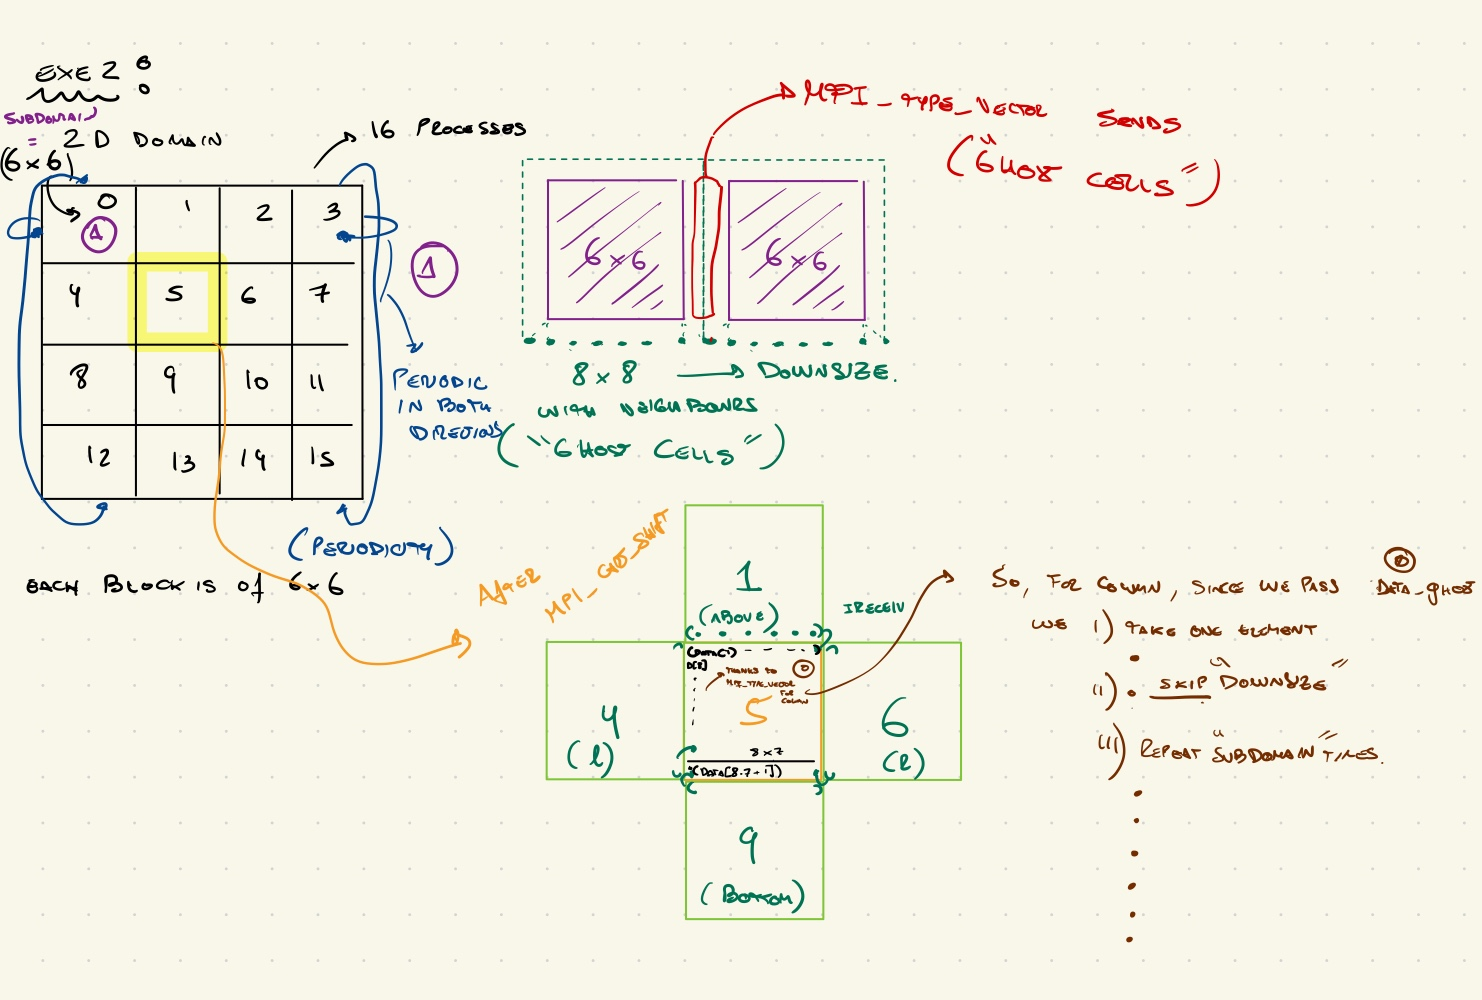
\includegraphics[width=\textwidth]{./img/exe2/draft.jpeg}
    \caption{Draft of the implementation}
  \end{figure}


To create a 2D MPI communicator (4x4) with periodic boundaries, I first set the dimensions of the grid as 4x4 and then set to true the periodic boundaries in both dimensions as required. 
This means that the end of one side will be connected to the beginning of the parallel side. After this variable definition, I use the $MPI\_Cart\_create$ function to create the communicator.
This function receives as input the MPI communicator, the number of dimensions, the dimensions of the grid, the periodic boundaries and a flag for reordering (we set it to false since we do not allow reordering).

To automatically manage the ranks of the neighboring processes, I use the $MPI\_Cart\_shift$ function. This function receives as input the communicator, the dimension in which we want to shift, the shift amount, and the ranks addresses 
of the neighboring processes where we want to store the ranks. We do this for vertical and horizontal neighbors.

Now, to manage the column vectors of ghost cells, we need to use the $MPI\_Type\_vector$ function. This function receives as input the number of elements in the block to send, the length of the block, the stride (how many elements to jump to the next block, which in our case 
is the $DOMAINSIZE$), the datatype, and stores the new datatype in the variable $data\_ghost$. After this, we need to commit the new datatype.
To understand the inputs of this function, we can observe the draft. We know we want to send $SUBDOMAIN$ elements that form the ghost cells for some process,
and as mentioned before, each element of the column would be at distance $DOMAINSIZE$ of each other. 

We can now implement the communication of the processes. First, as suggested, I use the $MPI\_Irecv()$, $MPI\_Send()$, $MPI\_Wait()$ functions to achieve this since it allows for a non-blocking communication.
I defined first the $irecv$ just to "post" the receives first, however, since it is non-blocking it should not make a difference. The input of the $MPI_Irecv$ are
Where we set the starting index, how many elements we want to receive ($SUBDOMAIN$), the datatype ($MPI\_DOUBLE$), the source (neighboring process), the tag (match with the sender tag), the communicator and the request variable \footnote{\url{https://rookiehpc.org/mpi/docs/mpi_irecv/index.html}}.

\begin{lstlisting}
    // From top -> count from 1 to 6 since the corners are not ghost cells for the receiver. 
    MPI_Irecv(&data[1], SUBDOMAIN, MPI_DOUBLE, rank_top, 0, comm_cart, &request[0]);
    // From bottom
    MPI_Irecv(&data[(DOMAINSIZE)*(DOMAINSIZE-1)+1], SUBDOMAIN, MPI_DOUBLE, rank_bottom, 1, comm_cart, &request[1]);
    // From left
    MPI_Irecv(&data[DOMAINSIZE], 1, data_ghost, rank_left, 2, comm_cart, &request[2]);
    // From right
    MPI_Irecv(&data[2*DOMAINSIZE-1], 1, data_ghost, rank_right, 3, comm_cart, &request[3]);

    // To top
    MPI_Isend(&data[DOMAINSIZE+1], SUBDOMAIN, MPI_DOUBLE, rank_top, 1, comm_cart, &request[4]);
    // To bottom
    MPI_Isend(&data[DOMAINSIZE*(DOMAINSIZE-2)+1], SUBDOMAIN, MPI_DOUBLE, rank_bottom, 0, comm_cart, &request[5]);
    // To left
    MPI_Isend(&data[DOMAINSIZE+1], 1, data_ghost, rank_left, 3, comm_cart, &request[6]);
    // To right
    MPI_Isend(&data[DOMAINSIZE+SUBDOMAIN], 1, data_ghost, rank_right, 2, comm_cart, &request[7]);
\end{lstlisting}

To figure out the indexing, the drafts helped. For example, we know that we will store the receiving bottom values of the $top$ rank in the 
first row (non corner value as starting value). We will store 6 ($SUBDOMAIN$) of them. From the bottom part, we know that the size of the 
block is $DOMAINSIZE$ X $DOMAINSIZE$ , therefore, ($DOMAINSIZE$ X ($DOMAINSIZE$-1))+1 leave us in the beginning of the last row, where we expect to
store the first row information of our $bottom$ rank. 

For the left column, the help of our previous $MPI\_Type\_vector$ definition comes on handy. We know that the rightmost column (ignoring corners always), will be 
the values to be received in our leftmost column. However, ignoring corner, this means that we point to $data[DOMAINSIZE]$ which is the beginning of the column. 
Then, the filling should be on $DOMAINSIZE$ jumps, which is manage by our $MPI\_Type\_vector$ definition (remember stride). 

The same logic applies to the right side, and for the sending part. 

Finally, we need to wait for the 8 responses before printing out the values of a specific rank. Therefore, we pass the counts to wait, the request and status to the $MPI\_Waitall$
function. After the printing is done, we free the created buffers for the columns and the communication with $MPI\_Type\_free$ and $MPI\_Comm\_free$ respectively.
\section{Task: Parallelizing the Mandelbrot set using MPI [20 Points]}
For implementing $createPartition$, i first initialized the dimensions of the grid and I set the periods to false since we do not want periodic boundaries.
Then, as suggested, i made use of the $MPI\_Dims\_create$ function to create the dimensions of the grid. \footnote{\url{https://rookiehpc.org/mpi/docs/mpi_dims_create/index.html}} This function receives the number of processes, the number of dimensions and the dimensions array, and
it will output how many processes we have in each dimension. I assigned this to $p.ny$ and $p.nx$ respectively. To create the Cartesian communicator, I follow a similar procedure as on previous exercise where I pass the initialized communicator, the number of dimensions, the dimensions of the grid in terms of processes, I do 
not allow for reordering and I set the periods to false. In addition, I store the new communicator in $p.comm$. Finally, I instantiate the coordinates of the current process in the grid with the $MPI\_Cart\_coords$ function, which determines the coordinates of the current process/rank in the grid accordingly
based on the communication environment, the rank of the process, the number of dimensions and the address to store the coordinates. \footnote{\url{https://rookiehpc.org/mpi/docs/mpi_cart_coords/index.html}}

With respect to $updatePartition$, after copying the old partition information, I use the $MPI\_Cart\_coords$ function to update the coordinates of the current process in the grid following the same logic as in the previous function.

With respect to $createDomain$, we need to translate how many pixels are assigned to each local process. For this, we divide the total number of pixels on each dimension by the number of processes in the corresponding dimension.
Then, we compute the index of the first pixel on each domain. For this, we can think of multiplying the process index in the corresponding dimension by the number of pixels per process. Such that if, for example, we have 
3 processes over the x-dim \footnote{As for example: $\frac{[Process 3], [Process 4], [Process 5]}{[Process 0], [Process 1], [Process 2]}$} with an image of 1000 pixels, the first process will take the first 333 pixels, the second one the next 333 and the last one the remaining 334 pixels.
Then, this can be simply calculated as $p.x * d.nx$ where $p.x$ is the x-coordinate of the process in the grid and $d.nx$ the number of pixels per process. 
Now, to calculate the last pixel, is simply as taking the start pixel, add the number of pixels per process and subtract one. 

To finally send the computations to the master process, I added $MPI\_Send$ such that any process that is not the master will send its local partition in a blocking manner such 
that everything it is sent before is received for the master to write the image. In addition, I free the memory allocated for the image and partition communicator.

\begin{figure}[H]
    \centering
    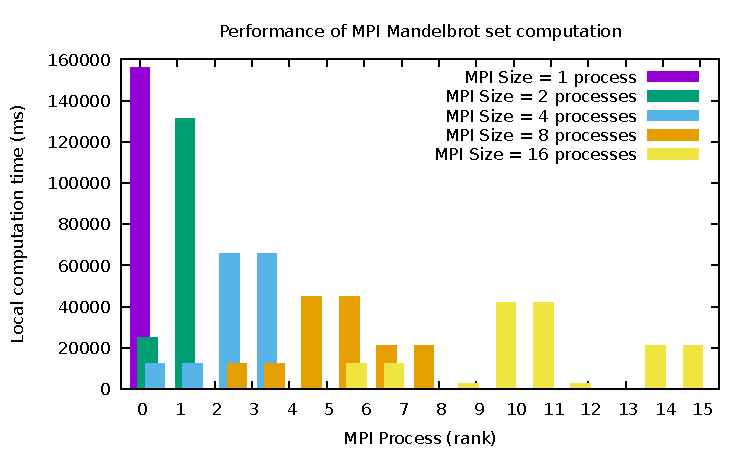
\includegraphics[width=\textwidth]{./img/exe3/perf.pdf}
    \caption{Performance graph}
  \end{figure}

What I observe is that the computation time is not balanced perfectly across processes for the same MPI size. I believe this happens because the computations over the mandelbrot set are not evenly distributed either
since the edges of the image tends to be less populated than, for example, the center-right part of the image. In any case, the computation time  is substantially improved by the parallelization in an apparent monotonic way although
not linearly. 

One possible improvement that emerge from this is to try to take into account the complexity of the different parts of the image when splitting the domain between processes.
Maybe we do not want perfect symmetric windows but adjusted by computation. 


\section{Task: Parallel matrix-vector multiplication and the power method [40 Points]}
\subsection{Implementation}
With respect to the code implementations, using the hint idea and the pre-defined variables I first calculate the "base" number of rows per process $n / size$ and the reminder 
that emerge from the given size and number of elements. Then, the idea is that for ranks under such reminder, as suggested by the hint when it mentions \textit{"The first "n \% size" processes get "n / size + 1" rows"},
the number of rows per process is incremented by one. Whereas, the rest of the ranks will have the "base" number of rows. For example,
if n = 11 and size = 4, rank 0 gets rows 0 to 2, rank 1 gets rows 3 to 5, rank 2 gets rows 6 to 8, rank 3 gets rows 9 to 10. In addition, I compute the beginning index of 
each as the $rank * (rows per process + 1)$ per each case in the less than reminder ranks. While the same variable would take (reminder * (rowsperprocess + 1)) + ((rank - reminder) * rowsperprocess) for the rest of processes. 
In this expression, the idea is that the first term skip the already assigned ones in the "less than reminder" case, and then, we add the start according to the rank position with respect to the reminder. 
For the end index is as simple as taking the beginning, adding the local rows and removing one. 

\begin{lstlisting}
    // Partition work evenly among processes
    int nrows_local = n;// how many rows each process will get
    int row_beg_local = 0;// starting row
    int row_end_local = row_beg_local + nrows_local - 1;
  
    // To do: Partition the "n" rows of the matrix evenly among the "size" MPI
    //        processes.
    // Hint : The first "n % size" processes get "n / size + 1" rows, while the
    //        remaining processes get "n / size".
    int rowsxproc = n / size;
    int remrows = n % size; //reminder 
    //destribution as required:
    if (rank < remrows) {
      nrows_local = rowsxproc + 1;
      row_beg_local = rank * (rowsxproc + 1); //if n = 11 and size = 4, rank 0 gets rows 0 to 2, rank 1 gets rows 3 to 5, rank 2 gets rows 6 to 8, rank 3 gets rows 9 to 10
    } else {
      nrows_local = rowsxproc;
      row_beg_local = (remrows * (rowsxproc + 1)) + ((rank - remrows) * rowsxproc); 
      //so in the first term i skip the already distributed ones, and then, i calculate the offset for the remaining ones, since those remainings would be over the reminder 
    }
\end{lstlisting}

For the broadcasting part \footnote{\url{https://rookiehpc.org/mpi/docs/mpi_bcast/index.html}}, I pass the vector to broadcast (y), the number of elements to broadcast (n), the datatype (MPI\_DOUBLE), 
the root process (0) and the communicator (MPI\_COMM\_WORLD).

Now, with respect to the actual block calculation to parallelize the power method. One key thing is to realize that we use $i_global$ to "store" the representation
of the process row in the actual full matrix whereas $i_local$ will work as a local indexing of that storage. Therefore, after the assigned vector to the process is normalized
we loop over it and store in a local y that will later be aggregated. 

\begin{lstlisting}
    for (int i_local = 0; i_local < nrows_local; ++i_local) {
        y_local[i_local] = 0.;    // Store in y_local, not y
        for (int j_global = 0; j_global < n; ++j_global) {
            y_local[i_local] += A[i_local*n + j_global]*v[j_global];  // Store in y_local, not y
        }
    } 
\end{lstlisting}

Once the local y is computed, I proceed to create a buffer that stores the amount of elements that each process will need to send 
and another one for storing the index where each data need to be stored when received.:

\begin{lstlisting}
    int* recv = (int*) calloc(size, sizeof(int)); 
    int* indices = (int*) calloc(size, sizeof(int)); 
\end{lstlisting}

That I proceed to fill with the same idea as in the beginning:

\begin{lstlisting}
    for (int i = 0; i < size; ++i) { 
        if (i < remrows) {
            recv[i] = rowsxproc + 1;
            indices[i] = i * (rowsxproc + 1);
        } else {
            recv[i] = rowsxproc;
            indices[i] = remrows * (rowsxproc + 1) + 
                        (i - remrows) * rowsxproc;
        }
      }
\end{lstlisting}

Meaning that, if for example n = 10 and size = 3 then, recv[0] = 4, recv[1] = 3, recv[2] = 3. And indices[0] = 0, indices[1] = 4, indices[2] = 7.
Then, we are ready to set up the "gathering": 

\begin{lstlisting}
    MPI_Allgatherv(y_local, nrows_local, MPI_DOUBLE, y, recv, indices, MPI_DOUBLE, MPI_COMM_WORLD);
\end{lstlisting}

Where we need to pass the local computations, then the elements the process is sending, the type, the global storage (y), how many elements comes from each process (recv),
the indices where to put each thing (indices), the data type of it, and the communicator. After this, we can free the recv and indices buffers. 

\subsection{Results}
\subsubsection{Strong Scaling and Multi-Nodes Strong Scaling}
For the same node strong scaling, I created a $strong\_scaling.sh$ script that, given the parameters of the cluster and a list of processes 
it proceeds to run the implemented code with the different elements of the mentioned list and store the results in a csv file that I run in the 
python file $strong\_plot.py$ with the following outcome: 

\begin{figure}[H]
    \centering
    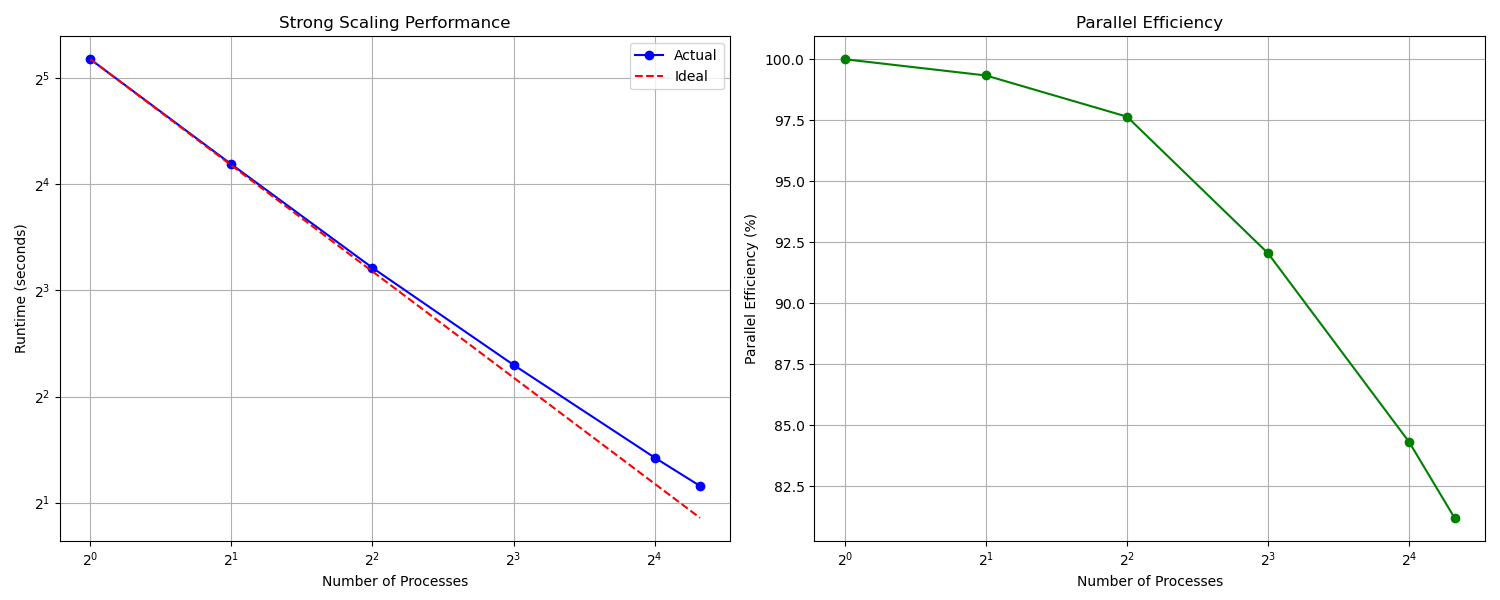
\includegraphics[width=\textwidth]{./img/exe4/strong_scaling.png}
    \caption{Strong Scaling in one Node}
  \end{figure}

\begin{table}[h!]
\centering
\begin{tabular}{|c|c|c|c|}
\hline
Processes & Runtime(s) & Speedup & Efficiency(\%) \\
\hline
1 & 36.22 & 1.000 & 100.00 \\
2 & 18.23 & 1.987 & 99.35 \\
4 & 9.27 & 3.91 & 97.64 \\
8 & 4.92 & 7.36 & 92.0432 \\
16 & 2.68 & 13.49 & 84.31 \\
20 & 2.23 & 16.24 & 81.19 \\
\hline
\end{tabular}
\caption{Strong scaling analysis with all processes on the same node}
\end{table}


Before commenting the results, is important to comment that I test the implementation in with a small matrix showing perfect performance in the different three cases.
However, and I assume by actual strong scaling analysis to be comparable, none converges with the given tolerance and iterations with these sizes which I suppose is reasonable for our 
testing purposes of strong and weak scaling. 

With respect to this first results, the performance is almost ideal, where ideal is calculated by taking the time of the baseline case (1 process) and dividing by the number of processes.
Whereas the actual parallel efficiency is calculated by taking the ratio of the single process with respect to the number of processes multiplied by the time taken by the case.  \footnote{\url{https://scicomp.ethz.ch/wiki/Parallel_efficiency}}

What we can see from the first plot is that the runtime is almost ideal, with a slight deviation starting from more than 4 processes, which I believe comes from similar reasons as we saw in previous assignments
with the Amdahl's law since the potential speedup that we can achieve is limited by the unavoidable sequential part of the program, which becomes "heavier" in the calculation when the parallelizable part is even faster. 
The parallel efficiency also correlates with the runtime graph but showing this slight off deviation even earlier. In any case, the performance is good (notice that the plot is in a logarithmic scale).

Now, for the multi-node strong scaling, I created a $multi\_strong\_scaling.sh$ script that, with the same logic but a different setup for the nodes where each node receives a task and the task is split into a maximum of 16 nodes 
accordingly to the process number count. Notice that runs to 16 since I did not have 20 available nodes for running on each of them separately: 

\begin{figure}[H]
    \centering
    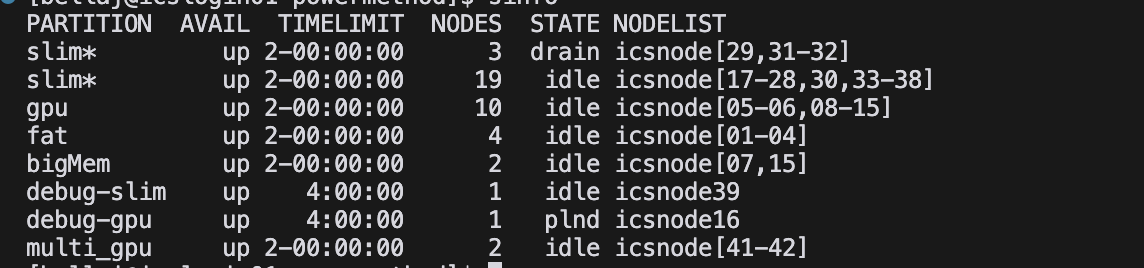
\includegraphics[width=\textwidth]{./img/exe4/nodes.png}
    \caption{Nodes availability}
  \end{figure}

I actually set it up to run on 19 but since we loop until 16 the later are never used.

With this in mind, the results are the following: 

\begin{figure}[H]
    \centering
    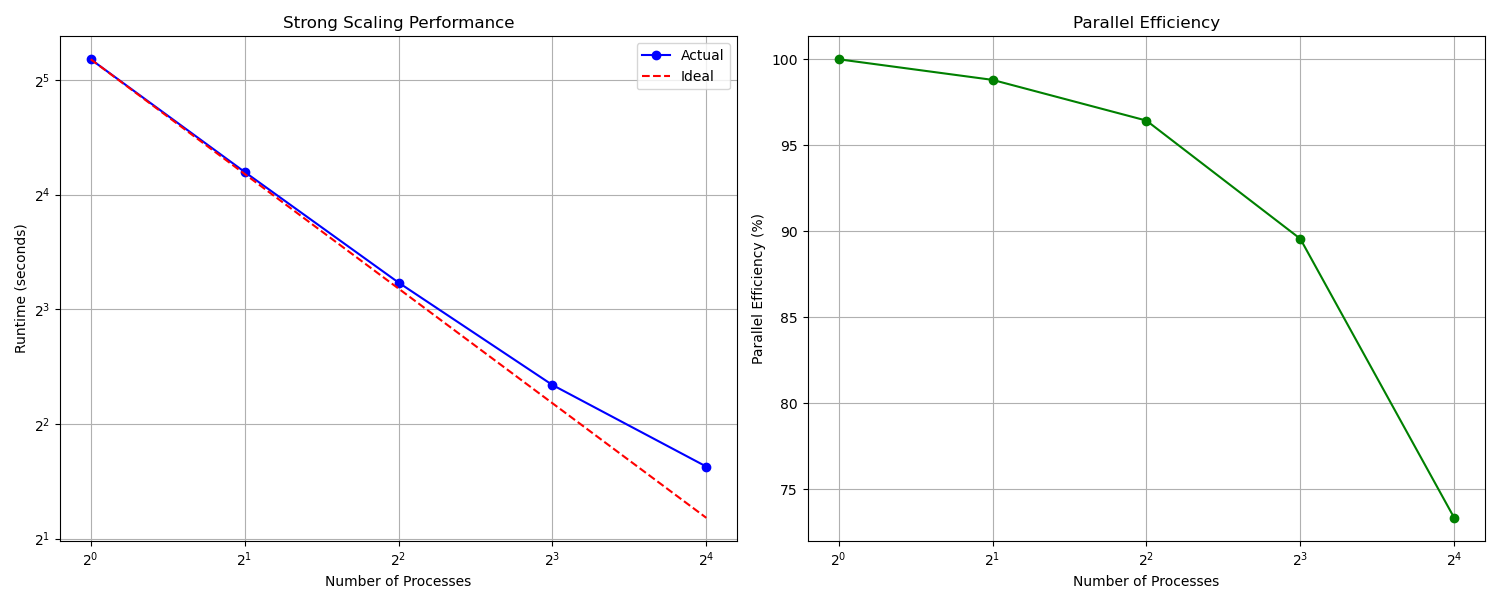
\includegraphics[width=\textwidth]{./img/exe4/strong_scaling-multi.png}
    \caption{Multi-Node Strong Scaling}
  \end{figure}

\begin{table}[h!]
\centering
\begin{tabular}{|c|c|c|c|}
\hline
Processes & Runtime(s) & Speedup & Efficiency(\%) \\
\hline
1 & 36.270 & 1.000 & 100.00 \\
2 & 18.355 & 1.976 & 98.80 \\
4 & 9.403 & 3.857 & 96.44 \\
8 & 5.062 & 7.165 & 89.56 \\
16 & 3.091 & 11.735 & 73.34 \\
\hline
\end{tabular}
\caption{Strong scaling analysis with each process in a different node}
\end{table}

With a slightly worse performance that on same nodes computations. This makes sense since
there is an implicit communication overhead for the inter-node case. In the intra-node case the communication
it is done through shared memory whereas in the inter-node case the communication is done through the network 
which typically is slower. In addition, in the same node case, the memory is shared, so it can be shared even cache lines 
which makes it even more fast. I suppose that this can even be aggravated with more users more nodes at the same time, which 
in the case of this measurement I was alone in the cluster. 

\subsubsection{Weak Scaling}
As before, i created a $weak\_scaling.sh$ script that, given the same cluster configuration and now, with the added matrix sizes for each
process number taking as base 10000, it proceeds to run the implemented code with the different elements of the mentioned list and store the results in a csv file that i run in the 
python file $plot.py$ with the following outcome: 

\begin{figure}[H]
    \centering
    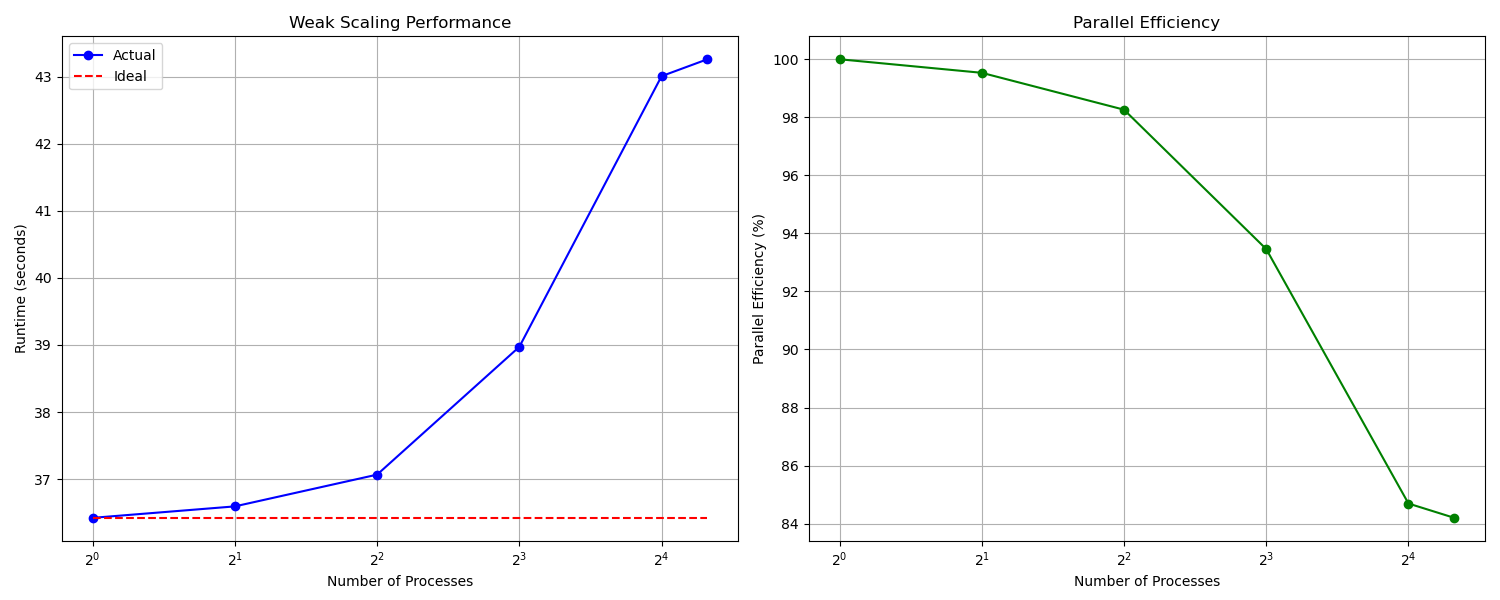
\includegraphics[width=\textwidth]{./img/exe4/weak_scaling.png}
    \caption{Weak Scaling}
  \end{figure}

\begin{table}[h!]
\centering
\begin{tabular}{|c|c|c|c|}
\hline
Processes & Size & Runtime(s) & Efficiency(\%) \\
\hline
1 & 10000 & 36.423 & 100.00 \\
2 & 14142 & 36.594 & 99.53 \\
4 & 20000 & 37.067 & 98.26 \\
8 & 28284 & 38.973 & 93.46 \\
16 & 40000 & 43.007 & 84.69 \\
20 & 44721 & 43.259 & 84.20 \\
\hline
\end{tabular}
\caption{Weak scaling analysis showing how runtime and efficiency change as both the number of processes and problem size increase proportionally}
\end{table}

Notice that the scaling of the matrix size is such that we keep constant the computation per process.
The results are comparable as previous ones, such that the runtime shows a slight misalignment with the ideal after the 4 process case. Notice that
the parallel efficiency is calculated as the ratio of the single process time with respect to the process time for the respective case since the scaling is 
done in the matrix size. Again, the numbers are quite good. 

For the multi-node weak scaling, the same problem happens when trying to achieve to run 20 processes, so I limited to 16:

\begin{figure}[H]
    \centering
    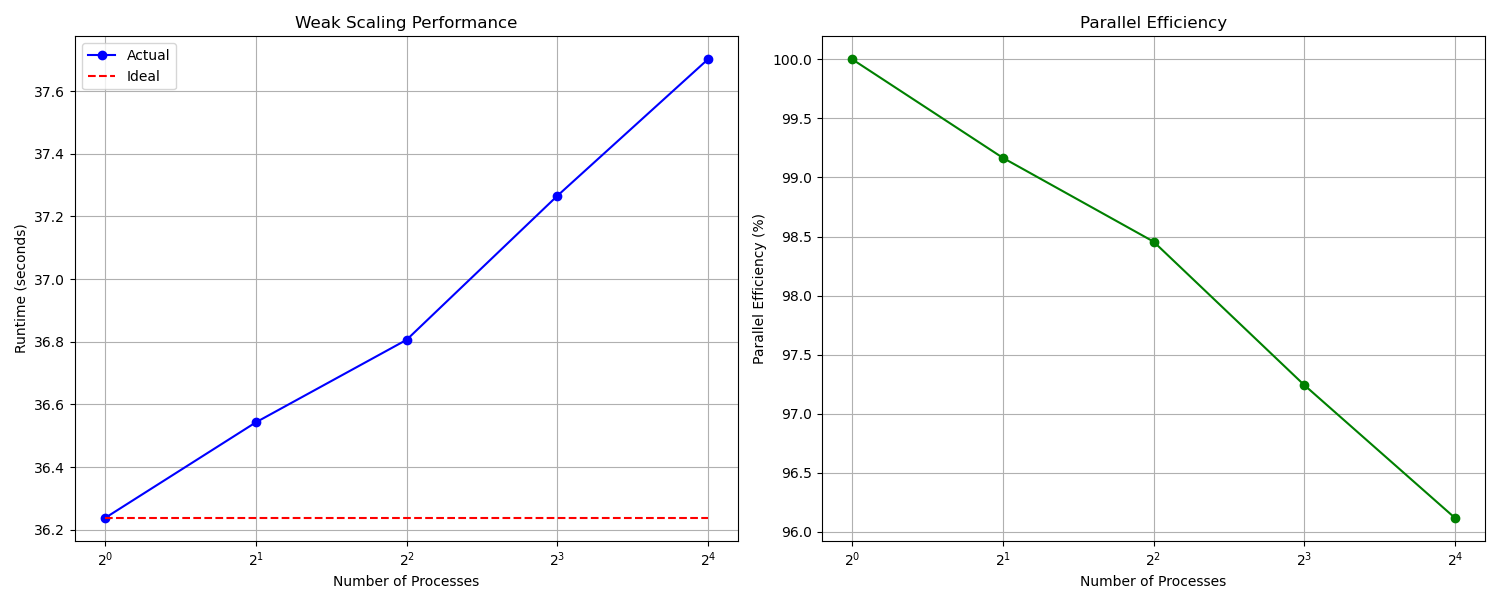
\includegraphics[width=\textwidth]{./img/exe4/weak_scaling_multi.png}
    \caption{Multi-Node Weak Scaling}
  \end{figure}

\begin{table}[h!]
\centering
\begin{tabular}{|c|c|c|c|}
\hline
Processes & Size & Runtime(s) & Efficiency(\%) \\
\hline
1 & 10000 & 36.238 & 100.00 \\
2 & 14142 & 36.543 & 99.17 \\
4 & 20000 & 36.806 & 98.46 \\
8 & 28284 & 37.265 & 97.24 \\
16 & 40000 & 37.701 & 96.12 \\
\hline
\end{tabular}
\caption{Multi-Node Weak scaling analysis showing how runtime and efficiency change as both the number of processes and problem size increase proportionally}
\end{table}

Surprisingly, the performance seems better for the multi node case with respect to same node case in weak scaling. 
Since the change lays in the matrix size then the difference should be or/and in the memory bandwidth or size. I suspect that since the 
shared memory bus has a fixed bandwidth were each process must compete for it, when data growth we can reach the peak of that bandwith 
whereas, in multinodes case, all nodes gets its own "data route" to drive in whose final speed can then compensate the distribution latency
later on.  

Therefore, to summarize between the two cases, in the strong scaling case, seems that performance is more affected by communication overheads than resources
since matrix size is constant whereas in weak scaling, the size of the matrix scales with the processes which means that the weight of the data bandwidth
became bigger than the communication overhead. 


\section{Task:  Quality of the Report [15 Points]}


\end{document}
